%-----------------------------------------------------------------------------%
\chapter{\topikSatu}
%-----------------------------------------------------------------------------%

%-----------------------------------------------------------------------------%
\section{Pendahuluan}
%-----------------------------------------------------------------------------%
Topik eksperimen pertama adalah perkalian matriks-vektor dan perkalian matriks bujur sangkar dengan beberbagai algoritma paralel. 

\subsection{Perkalian Matriks-Vektor} 

\subsubsection{Row-Wise Decomposition}

Algoritma paralel perkalian matriks-vektor yang paling sederhana, yaitu memecah proses perkalian berdasarkan baris matriks (\f{row-wise}). Setiap prosesor akan bertanggung jawab untuk mengalikan sebuah baris matriks dan vektor pada satu waktu. Jika jumlah prosesor ($np$) lebih sedikit dari jumlah baris matriks ($r$) maka setiap prosesor bertugas mengalikan $n = \frac{r}{np}$ secara sekuensial.

\begin{figure}
	\centering
	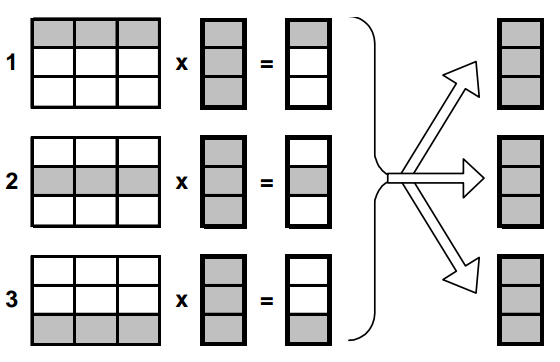
\includegraphics[width=0.75\textwidth]
	{pics/mv_rowwise}
	\caption{Perkalian matriks-vektor Row-Wise Decomposition}
	\label{fig:mv_rowwise}
\end{figure}  

\subsubsection{Column-wise Decomposition}

Algoritma perkalian matriks-vektor ini merupakan alternatif dari \f{row-wise decomposition} di mana pemecahan proses perkalian dilakukan berdasarkan kolom matriks. Setiap proses akan mengalikan sebuah kolom matriks dan sebuah elemen vektor pada satu waktu. Mirip dengan algoritma \f{row-wise decomposition}, jika jumlah prosesor ($np$) lebih sedikit dari jumlah kolom matriks ($c$) maka setiap prosesor bertugas mengalikan $n = \frac{c}{np}$ secara sekuensial.

\begin{figure}
	\centering
	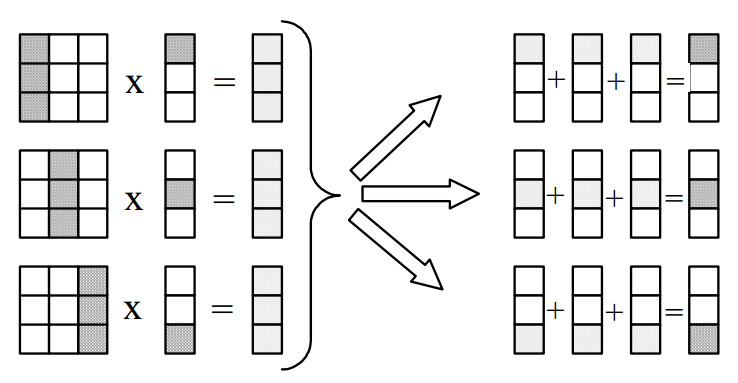
\includegraphics[width=0.9\textwidth]
	{pics/mv_colwise}
	\caption{Perkalian matriks-vektor Column-Wise Decomposition}
	\label{fig:mv_colwise}
\end{figure}  

\subsubsection{Checkerboard Decomposition}

Algoritma perkalian matriks-vektor \f{checkerboard decomposition} ini membagi matriks menjadi submatriks dengan ukuran yang sama dan mengalikannya dengan subvektor yang sesuai. Hasil perkalian tersebut kemudian akan dijumlahkan dan dipetakan ke vektor hasil.

Prekondisi dari algoritma ini adalah jumlah elemen matriks ($n$) harus bisa dibagi rata ke sejumlah prosesor ($np$) atau dengan kata lain memenuhi persamaan \ref{eq:mv_checkerboard}. Hasil pembagian ini ($x$) akan menjadi ukuran submatriks (dan subvektor) yang dikerjakan di tiap proses secara paralel.

\begin{equation}
	x = \sqrt{\frac{n}{np}},\text{ where } x \in \mathbb{Z}
	\label{eq:mv_checkerboard}
\end{equation}


\begin{figure}
	\centering
	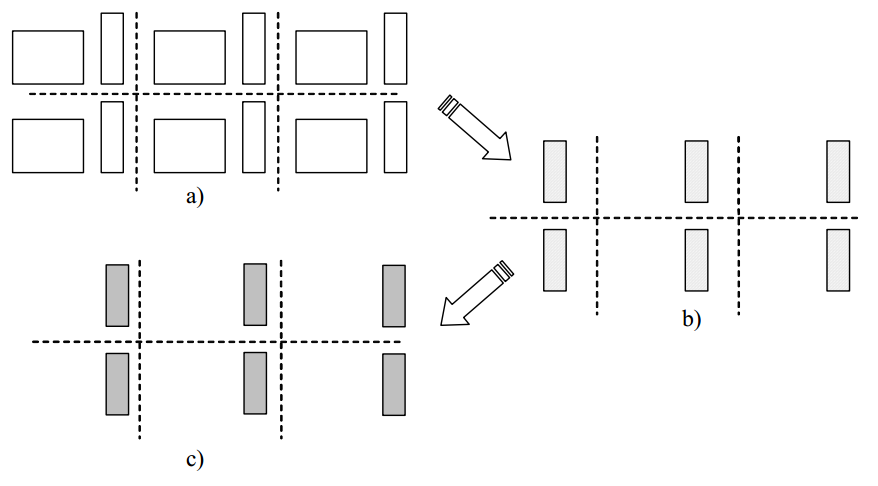
\includegraphics[width=0.75\textwidth]
	{pics/mv_checkerboard}
	\caption{Perkalian matriks-vektor Checkerboard Decomposition}
	\label{fig:mv_checkerboard}
\end{figure}  

\subsection{Perkalian Matriks Bujursangkar} 

\subsubsection{Row-Wise Decomposition}

Mirip dengan algoritma perkalian matriks-vektor \f{row-wise decomposition}, algortima ini juga membagi pekerjaan berdasarkan baris dari matriks pertama seperti yang diilustrasikan pada gambar \ref{fig:mm_rowwise}. Setiap prosesor akan mengalikan sebuah baris dari matriks pertama $A$ dengan seluruh kolom dari matriks kedua $B$. Hasil dari seluruh prosesor kemudian dikonkatenasi menjadi matriks baru $C$.

\begin{figure}
	\centering
	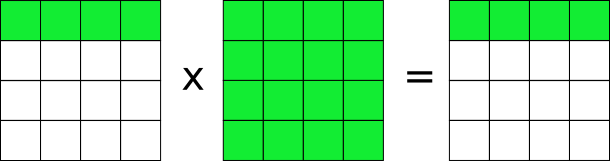
\includegraphics[width=1\textwidth]
	{pics/mm_rowwise}
	\caption{Perkalian matriks bujursangkar Row-Wise Decomposition}
	\label{fig:mm_rowwise}
\end{figure}

\subsubsection{Cannon}

Algoritma Cannon menggunakan dekomposisi seperti algortima matriks-vektor \f{checkerboard decomposition} di mana matriks $A$ dan $B$ dibagi menjadi menjadi submatriks bujursangkar. Perbedaan pada algoritma Cannon adalah prekondisi di mana jumlah proses ($np$) harus merupakan bujursangkar sempurna (\f{perfect square}). Tujuan utama dari algoritma ini adalah untuk meningkatkan efisiensi penggunaan memori pada proses paralel.

\begin{figure}
	\centering
	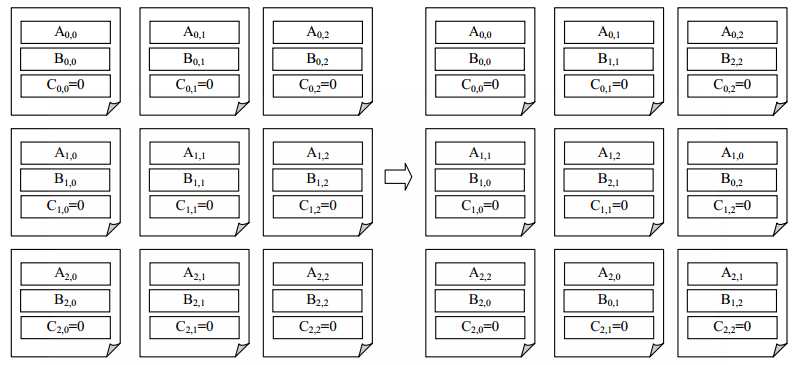
\includegraphics[width=1\textwidth]
	{pics/mm_cannon}
	\caption{Perkalian matriks bujursangkar Cannon}
	\label{fig:mm_cannon}
\end{figure}

\subsubsection{Fox}

Algoritma Fox memiliki kemiripan dengan algoritma Cannon dalam hal dekomposisi matriks menjadi submatriks bujursangkar dan pemetaan prosesor yang harus dapat membentuk bujursangkar sempurna (\f{perfect square}). Yang membedakan algoritma Fox dan Cannon adalah skema distribusi awal submatriks ke prosesor

\begin{figure}
	\centering
	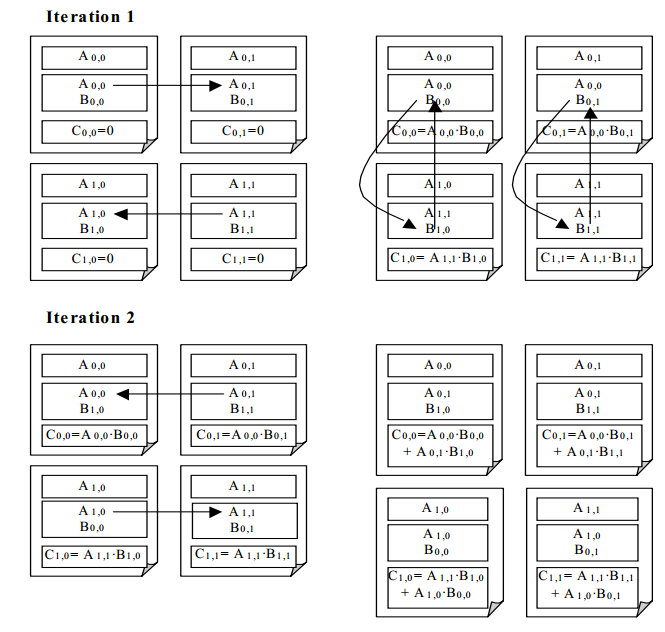
\includegraphics[width=0.75\textwidth]
	{pics/mm_fox}
	\caption{Perkalian matriks bujursangkar Fox}
	\label{fig:mm_fox}
\end{figure}

\subsubsection{DNS}

Algoritma yang diberi nama berdasarkan nama pembuatnya (Dekel, Nassimi and Aahni) ini, diajukan dalam rangka meningkatkan lagi efisiensi penggunaan memori pada perkalian matriks bujursangkar secara paralel. Karakteristik algoritma ini adalah:
\begin{itemize}
	\item Berdasarkan partisi \f{intermediate data}
	\item Melakukan perkalian skalar $n^3$ sehingga membutuhkan proses sebanyak $n \times n \times n$
	\item Membutuhkan waktu komputasi $O(\log n)$ dengan menggunakan $O(\frac{n^3}{\log n})$
\end{itemize}

\begin{figure}
	\centering
	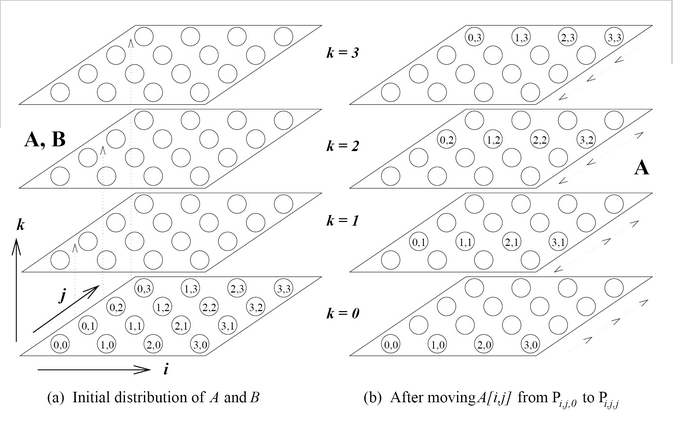
\includegraphics[width=1\textwidth]
	{pics/mm_dns1}
	\caption{Perkalian matriks bujursangkar DNS iterasi 1}
	\label{fig:mm_dns1}
\end{figure}

\begin{figure}
	\centering
	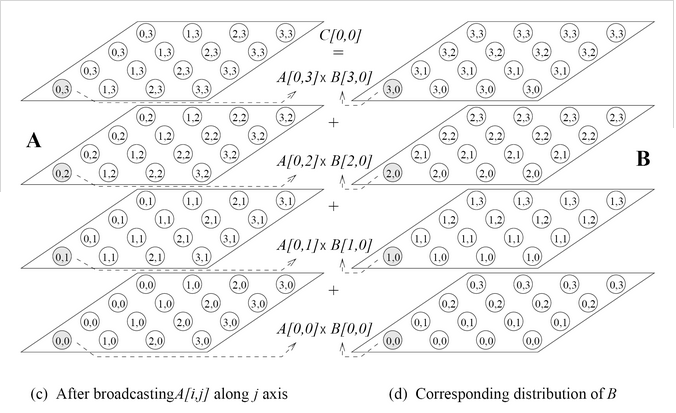
\includegraphics[width=1\textwidth]
	{pics/mm_dns2}
	\caption{Perkalian matriks bujursangkar DNS iterasi 2}
	\label{fig:mm_dns2}
\end{figure}


%-----------------------------------------------------------------------------%
\section{Eksperimen}
%-----------------------------------------------------------------------------%

\subsection{Perkalian Matriks-Vektor} 

\subsubsection{Row-Wise Decomposition}

Deskripsi program yang digunakan:
\begin{itemize}
	\item Sumber kode: \texttt{\url{ https://github.com/yohanesgultom/parallel-programming-assignment/blob/master/problem1/mv_rowwise.c}}
	\item Satu prosesor berlaku sebagai \manager dan sisanya berperan sebagai \worker 
	\item Tugas \manager adalah menginisialisasi matriks dan vektor, mendistribusikannya secara \f{row-wise decomposition} menggunakan \verb|MPI_Send| dan \verb|MPI_Bcast| dan mengumpulkan hasil dari tiap \worker dengan \verb|MPI_Recv|	
	\item Waktu eksekusi dan komunikasi dihitung (dalam detik) menggunakan \verb|MPI_Wtime|
\end{itemize}

Eksperimen dilakukan di \cluster UCSD dan Fasilkom dengan variasi jumlah prosesor di mana waktu yang diukur adalah nilai rata-rata dari lima kali eksekusi.

\begin{figure}
	\centering
	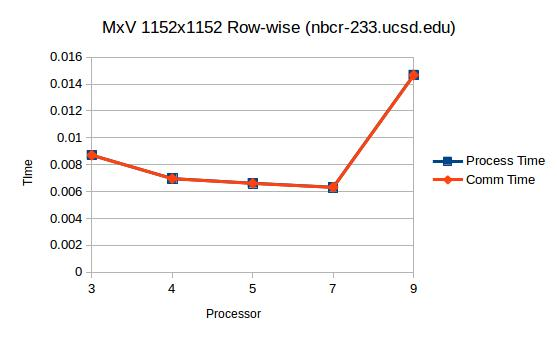
\includegraphics[width=1\textwidth]
	{pics/chart_mv_rowwise_nbcr}
	\caption{Grafik hasil eksperimen Row-Wise Decomposition cluster UCSD}
	\label{fig:result_mv_rowwise_nbcr}
\end{figure}  

\begin{figure}
	\centering
	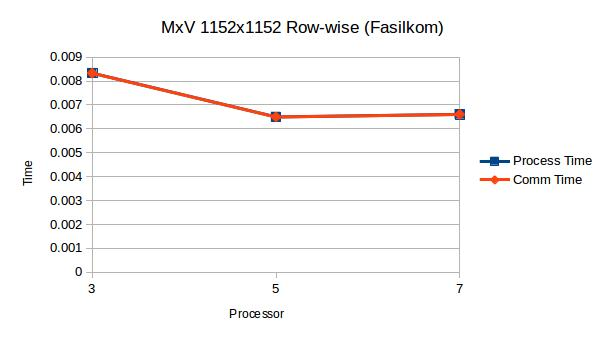
\includegraphics[width=1\textwidth]
	{pics/chart_mv_rowwise_fasilkom}
	\caption{Grafik hasil eksperimen Row-Wise Decomposition cluster Fasilkom UI}
	\label{fig:result_mv_rowwise_fasilkom}
\end{figure}  

Pada grafik gambar \ref{fig:result_mv_rowwise_nbcr}, terlihat bahwa pada \cluster UCSD terjadi penurunan waktu eksekusi/komunikasi (\speedup) ketika digunakan 3, 4, 5, 7 prosesor (2, 3, 4, 6 \worker). Tapi ketika digunakan 9 prosesor (8 \worker), waktu yang dibutuhkan malah meningkat (tidak terjadi \speedup). Kami tidak mencoba lebih dari 9 prosesor karena sepertinya hasilnya akan sama (tidak ada \speedup).

Sedangkan pada \cluster Fasilkom UI, kami hanya mencoba 3, 5, 7 prosesor karena masalah \f{permission} yang mengakibatkan hanya satu \node (8 prosesor) yang bisa digunakan. Seperti yang terlihat pada grafik gambar \ref{fig:result_mv_rowwise_fasilkom}, \speedup hanya terjadi pada prosesor 3-5. Sedangkan dari 5-7 prosesor tidak terjadi \speedup (waktu ekskusi hampir sama).

\subsubsection{Column-wise Decomposition}

Deskripsi program yang digunakan:
\begin{itemize}
	\item Sumber kode: \texttt{\url{ https://github.com/yohanesgultom/parallel-programming-assignment/blob/master/problem1/mv_columnwise.c}}
	\item Satu prosesor berlaku sebagai \manager dan sisanya berperan sebagai \worker 
	\item Tugas \manager adalah menginisialisasi matriks dan vektor, mendistribusikannya secara \f{column-wise decomposition} menggunakan \verb|MPI_Send| dan \verb|MPI_Bcast| dan mengumpulkan hasil dari tiap \worker dengan \verb|MPI_Recv|	
	\item Waktu eksekusi dan komunikasi dihitung (dalam detik) menggunakan \verb|MPI_Wtime|
\end{itemize}

Eksperimen dilakukan di \cluster UCSD dan Fasilkom dengan variasi jumlah prosesor di mana waktu yang diukur adalah nilai rata-rata dari lima kali eksekusi.

\begin{figure}
	\centering
	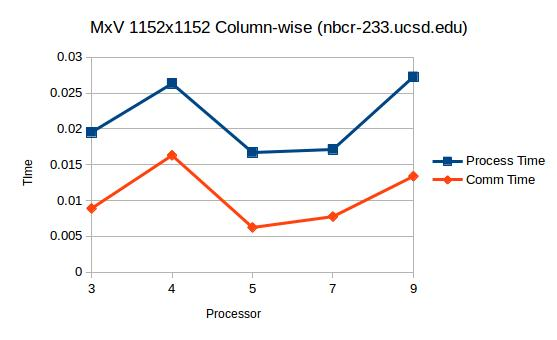
\includegraphics[width=1\textwidth]
	{pics/chart_mv_colwise_nbcr}
	\caption{Grafik hasil eksperimen Column-Wise Decomposition cluster UCSD}
	\label{fig:result_mv_colwise_nbcr}
\end{figure}  

\begin{figure}
	\centering
	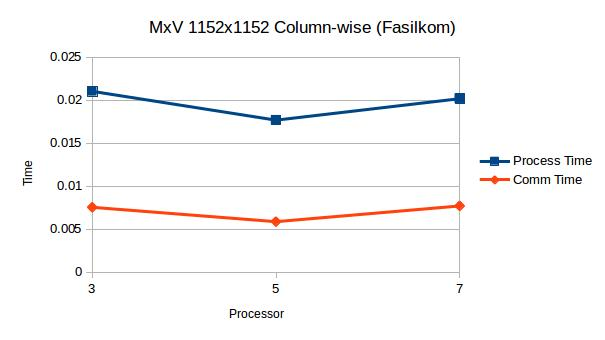
\includegraphics[width=1\textwidth]
	{pics/chart_mv_colwise_fasilkom}
	\caption{Grafik hasil eksperimen Column-Wise Decomposition cluster Fasilkom UI}
	\label{fig:result_mv_colwise_fasilkom}
\end{figure}  

Pada grafik gambar \ref{fig:result_mv_colwise_nbcr}, terlihat bahwa pada \cluster UCSD terjadi penurunan waktu eksekusi/komunikasi (\speedup) ketika digunakan 4-5 prosesor. Tapi ketika digunakan 3-4, 5-9 prosesor, waktu yang dibutuhkan malah meningkat (tidak terjadi \speedup).

Sedangkan pada \cluster Fasilkom UI, kami hanya mencoba 3, 5, 7 prosesor karena masalah \f{permission} yang mengakibatkan hanya satu \node (8 prosesor) yang bisa digunakan. Seperti yang terlihat pada grafik gambar \ref{fig:result_mv_colwise_fasilkom}, \speedup hanya terjadi pada prosesor 3-5. Sedangkan dari 5-7 prosesor tidak terjadi \speedup (waktu ekskusi meningkat).

\subsubsection{Checkerboard Decomposition}

Deskripsi program yang digunakan:
\begin{itemize}
	\item Sumber kode: \texttt{\url{ https://github.com/yohanesgultom/parallel-programming-assignment/blob/master/problem1/mv_checkerboard.c}}
	\item Satu prosesor berlaku sebagai \manager dan sisanya berperan sebagai \worker 
	\item Tugas \manager adalah menginisialisasi matriks dan vektor, mendistribusikannya secara \f{checkerboard decomposition} menggunakan \verb|MPI_Send| dan \verb|MPI_Bcast| dan mengumpulkan hasil dari tiap \worker dengan \verb|MPI_Recv|	
	\item Waktu eksekusi dan komunikasi dihitung (dalam detik) menggunakan \verb|MPI_Wtime|
\end{itemize}

Eksperimen dilakukan di \cluster UCSD dan Fasilkom dengan variasi jumlah prosesor di mana waktu yang diukur adalah nilai rata-rata dari lima kali eksekusi. Sedangkan pada \cluster Rocks hanya dilakukan perbandingan algoritma.

\begin{figure}
	\centering
	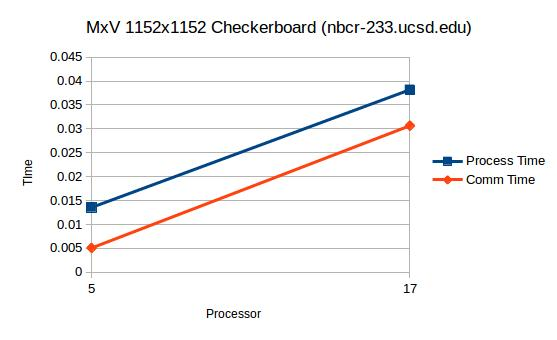
\includegraphics[width=1\textwidth]
	{pics/chart_mv_checkerboard_nbcr}
	\caption{Grafik hasil eksperimen Checkerboard cluster UCSD}
	\label{fig:result_mv_checkerboard_nbcr}
\end{figure}  

\begin{figure}
	\centering
	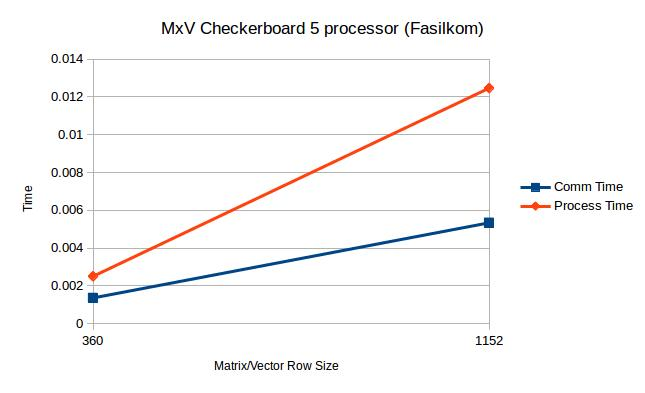
\includegraphics[width=1\textwidth]
	{pics/chart_mv_checkerboard_fasilkom}
	\caption{Grafik hasil eksperimen Checkerboard cluster Fasilkom UI}
	\label{fig:result_mv_checkerboard_fasilkom}
\end{figure}  

Pada grafik gambar \ref{fig:result_mv_checkerboard_nbcr}, terlihat bahwa waktu yang dibutuhkan malah meningkat (tidak terjadi \speedup) ketika kami meningkatkan jumlah prosesor dari 5-7. Kami tidak mencoba prosesor yang lebih banyak karena melihat pola yang sama (tidak ada \speedup).

Sedangkan pada \cluster Fasilkom UI, kami hanya mencoba 5 prosesor karena masalah \f{permission} yang mengakibatkan hanya satu \node (8 prosesor) yang bisa digunakan. Seperti yang terlihat pada grafik gambar \ref{fig:result_mv_checkerboard_fasilkom}, kami hanya mencoba melakukan eksekusi dengan ukuran matriks/vektor yang berbeda (360x360 dan 1152x1152).

\begin{figure}
	\centering
	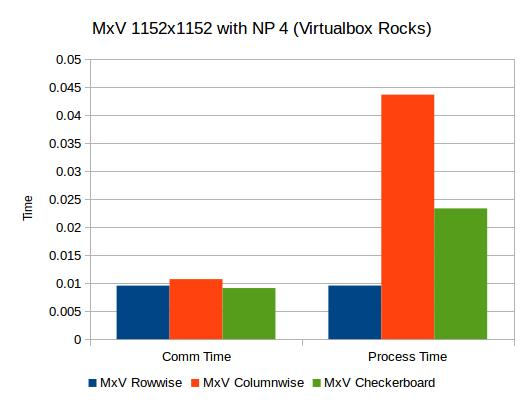
\includegraphics[width=1\textwidth]
	{pics/chart_mv_comparison_rocks}
	\caption{Grafik hasil eksperimen di cluster Rocks}
	\label{fig:result_mv_comparison_rocks}
\end{figure}  

Pada \cluster Rocks kami mengamati perbandingan kinerja dari tiga algoritma yang sudah di bahas. Sesuai dengan grafik pada gambar \ref{fig:result_mv_comparison_rocks}, hasil tercepat diperoleh dari algoritma \f{row-wise decomposition}. Kami tidak melakukan eksperimen dengan jumlah prosesor yang berbeda pada \cluster Rocks karena keterbatasan jumlah prosesor pada \f{laptop} yang kami gunakan.

\subsection{Perkalian Matriks Bujursangkar} 

\subsubsection{Row-Wise Decomposition}

Deskripsi program yang digunakan:
\begin{itemize}
	\item Sumber kode: \texttt{\url{ https://github.com/yohanesgultom/parallel-programming-assignment/blob/master/problem1/mm_rowwise.c}}
	\item Satu prosesor berlaku sebagai \manager dan sisanya berperan sebagai \worker 
	\item Tugas \manager adalah menginisialisasi dua buah matriks bujursangkar, mendistribusikannya secara \f{row-wise decomposition} menggunakan \verb|MPI_Send| dan \verb|MPI_Bcast| dan mengumpulkan hasil dari tiap \worker dengan \verb|MPI_Recv|	
	\item Waktu eksekusi dan komunikasi dihitung (dalam detik) menggunakan \verb|MPI_Wtime|
\end{itemize}

Eksperimen dilakukan di \cluster UCSD dan Fasilkom dengan variasi jumlah prosesor di mana waktu yang diukur adalah nilai rata-rata dari lima kali eksekusi.

\begin{figure}
	\centering
	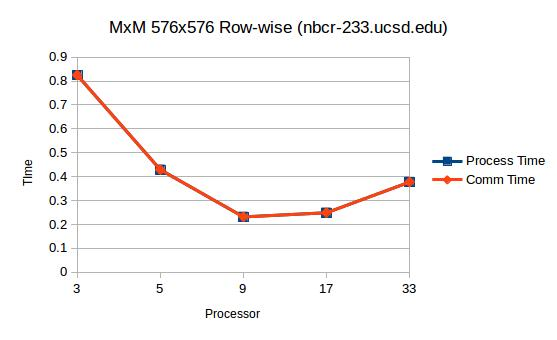
\includegraphics[width=1\textwidth]
	{pics/chart_mm_rowwise_nbcr}
	\caption{Grafik hasil eksperimen Row-Wise Decomposition cluster UCSD}
	\label{fig:result_mm_rowwise_nbcr}
\end{figure}  

\begin{figure}
	\centering
	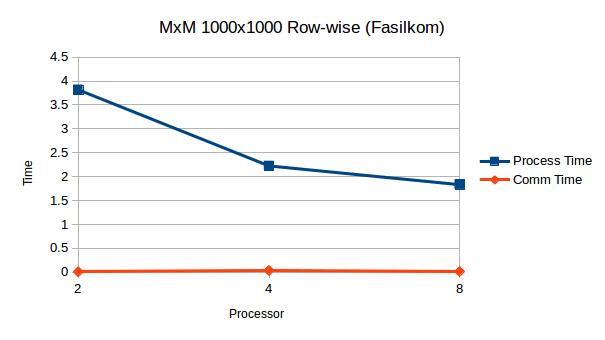
\includegraphics[width=1\textwidth]
	{pics/chart_mm_rowwise_fasilkom}
	\caption{Grafik hasil eksperimen Row-Wise Decomposition cluster Fasilkom UI}
	\label{fig:result_mm_rowwise_fasilkom}
\end{figure}

Pada grafik gambar \ref{fig:result_mm_rowwise_nbcr}, terlihat bahwa pada \cluster UCSD terjadi penurunan waktu eksekusi/komunikasi (\speedup) ketika digunakan 3-9 prosesor (2-7 \worker). Tapi ketika digunakan 17 prosesor (16 \worker), waktu yang dibutuhkan malah meningkat (tidak terjadi \speedup)

Sedangkan pada \cluster Fasilkom UI, kami hanya mencoba 2, 4, 8 prosesor karena masalah \f{permission} yang mengakibatkan hanya satu \node (8 prosesor) yang bisa digunakan. Seperti yang terlihat pada grafik gambar \ref{fig:result_mm_rowwise_fasilkom}, \speedup terjadi di seluruh eksperimen (pada prosesor 2-8).

\subsubsection{Cannon}

Deskripsi program yang digunakan:
\begin{itemize}
	\item Sumber kode: \texttt{\url{ https://github.com/yohanesgultom/parallel-programming-assignment/blob/master/problem1/mm_cannon.c}}
	\item Satu prosesor berlaku sebagai \manager tapi sekaligus \worker sedangkan sisanya hanya berperan sebagai \worker 
	\item Tugas \manager adalah menginisialisasi dua buah matriks bujursangkar, mempersiapkan topologi proses kartesian dengan \verb|MPI_Cart_create|, mendistribusikan pekerjaan dengan \verb|MPI_Sendrecv_replace| dan \verb|MPI_Cart_shift| untuk menentukan destinasi proses
	\item Waktu eksekusi dan komunikasi dihitung (dalam detik) menggunakan \verb|MPI_Wtime|
\end{itemize}

Percobaan hanya dilakukan di \cluster UCSD karena variasi jumlah prosesor harus bersifat \f{perfect square}, yaitu 4, 9, 16 dan 36. 

\begin{figure}
	\centering
	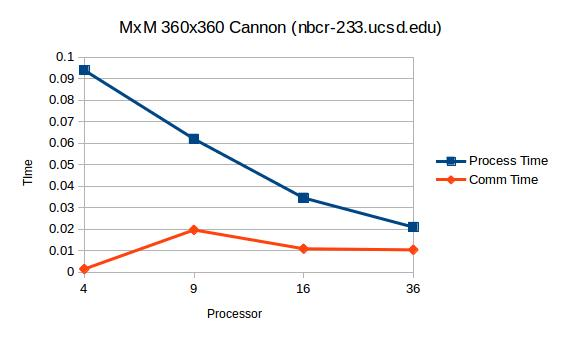
\includegraphics[width=1\textwidth]
	{pics/chart_mm_cannon_nbcr}
	\caption{Grafik hasil eksperimen algoritma Cannon cluster UCSD}
	\label{fig:result_mm_cannon_nbcr}
\end{figure}  

Seperti yang terlihat pada grafik gambar \ref{fig:result_mm_cannon_nbcr}, terjadi \speedup pada penambahan prosesor 4-36. Selain itu juga terlihat bahwa waktu komunikasi memiliki proporsi yang lebih sedikit dibandingkan dengan proporsi pada algoritma \f{row-wise decomposition}.

\subsubsection{Fox}

Deskripsi program yang digunakan:
\begin{itemize}
	\item Sumber kode: \texttt{\url{ https://github.com/yohanesgultom/parallel-programming-assignment/blob/master/problem1/mm_fox.c}}
	\item Satu prosesor berlaku sebagai \manager tapi sekaligus \worker sedangkan sisanya hanya berperan sebagai \worker 
	\item Tugas \manager adalah menginisialisasi dua buah matriks bujursangkar, mempersiapkan topologi proses kartesian dengan \verb|MPI_Cart_create|, mendistribusikan pekerjaan dengan \verb|MPI_Sendrecv_replace| dan \verb|MPI_Cart_shift| untuk menentukan destinasi proses
	\item Waktu eksekusi dan komunikasi dihitung (dalam detik) menggunakan \verb|MPI_Wtime|
\end{itemize}

Percobaan hanya dilakukan di \cluster UCSD karena variasi jumlah prosesor harus bersifat \f{perfect square}, yaitu 4, 9, 16 dan 36. 

\begin{figure}
	\centering
	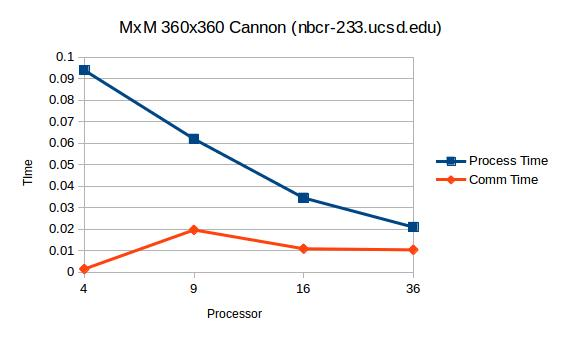
\includegraphics[width=1\textwidth]
	{pics/chart_mm_cannon_nbcr}
	\caption{Grafik hasil eksperimen algoritma Fox cluster UCSD}
	\label{fig:result_mm_fox_nbcr}
\end{figure}  

Seperti yang terlihat pada grafik gambar \ref{fig:result_mm_fox_nbcr}, terjadi \speedup pada penambahan prosesor 4-36. Selain itu juga terlihat bahwa waktu komunikasi memiliki proporsi yang lebih sedikit dibandingkan dengan proporsi pada algoritma \f{row-wise decomposition}.

\begin{figure}
	\centering
	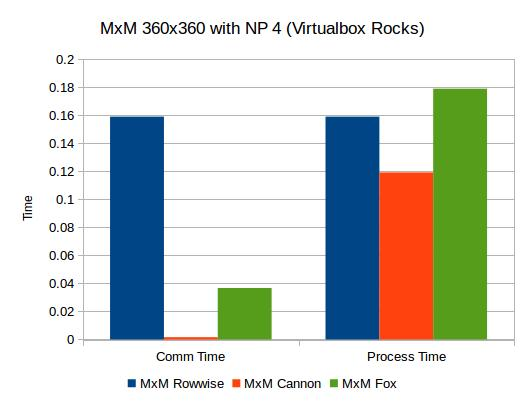
\includegraphics[width=1\textwidth]
	{pics/chart_mm_comparison_rocks}
	\caption{Grafik perbandingan algoritma pada cluster Rocks}
	\label{fig:result_mm_comparison_rocks}
\end{figure}  

Pada \cluster Rocks, kami mencoba membandingkan waktu proses antara algoritma \f{row-wise decomposition}, Cannon dan Fox dengan 4 prosesor. Hasil percobaan menunjukkan waktu proses dan komunikasi terendah dihasilkan oleh algoritma Cannon.

\subsubsection{DNS}

Deskripsi program yang digunakan:
\begin{itemize}
	\item Sumber kode: \texttt{\url{https://github.com/yohanesgultom/parallel-programming-assignment/blob/master/dns/dns.c}}
	\item Jumlah prosesor ($np$) harus memenuhi $x = \sqrt[3]{np}$ di mana $x \in \mathbb{Z}$
\end{itemize}

Eksperimen dilakukan dengan prosesor 8, 27 di \cluster UCSD dan 8 prosesor di \cluster Fasilkom UI,

\begin{figure}
	\centering
	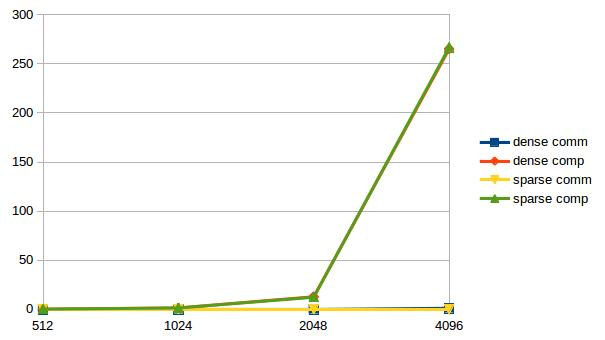
\includegraphics[width=1\textwidth]
	{pics/chart_mm_dns_nbcr_8}
	\caption{Grafik hasil eksperimen algoritma DNS degan 8 prosesor cluster UCSD}
	\label{fig:result_dns_nbcr_8}
\end{figure}  

\begin{figure}
	\centering
	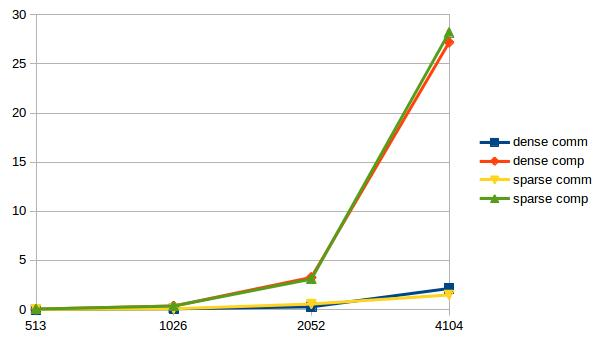
\includegraphics[width=1\textwidth]
	{pics/chart_mm_dns_nbcr_27}
	\caption{Grafik hasil eksperimen algoritma DNS degan 27 prosesor cluster UCSD}
	\label{fig:result_dns_nbcr_27}
\end{figure}  

Hasil percobaan pada \cluster UCSD yang ditunjukkan oleh grafik pada gambar \ref{fig:result_dns_nbcr_8} dan \ref{fig:result_dns_nbcr_27} menunjukkan bahwa proporsi waktu komunikasi hanya sedikit meningkat ketika ukuran matriks diperbesar. Dengan membandingkan dua grafik tersebut kita juga melihat adanya \speedup, khususnya pada ukuran matriks di atas 2048.

\begin{figure}
	\centering
	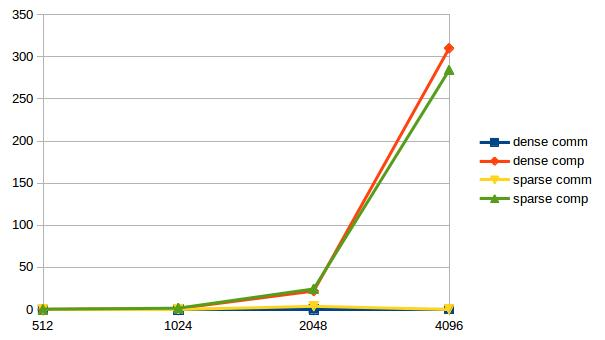
\includegraphics[width=1\textwidth]
	{pics/chart_mm_dns_fasilkom_8}
	\caption{Grafik hasil eksperimen algoritma DNS degan 8 prosesor cluster Fasilkom UI}
	\label{fig:result_dns_fasilkom_8}
\end{figure}  

\section{Kesimpulan}

Berdasarkan seluruh eksperimen pada topik ini, kami mengambil beberapa kesimpulan:

\begin{enumerate}
	\item Algoritma paralel dapat mengurangi waktu komputasi total (terjadi \speedup) khususnya pada algoritma yang proporsi waktu komunikasinya sedikit (Cannon, Fox, DNS)
	\item \Speedup akan semakin terlihat jika jumlah data semakin besar
	\item Pembagian bobot pekerjaan (\f{load balancing}) mempengaruhi kinerja algoritma paralel karena itu perlu disesuaikan perbandingan ukuran data dan jumlah prosesor yang digunakan
	\item Jika jumlah prosesor terus ditingkatkan, algoritma paralel akan mencapai titik jenuh (tidak terjadi \speedup lagi)
	\item Terdapat algoritma paralel didesain untuk kasus spesifik (matriks bujursangkar, matriks \f{dense/sparse}, jumlah prosesor \f{perfect square}) 
\end{enumerate}

